\begin{exercice*}    
    Un commerçant vend des tee-shirts à \Prix{5} l'unité. Les cinq derniers jours du mois de juillet, il lance une
    promotion de fin de saison : il vend ces tee-shirts par 3, au prix de \Prix{12} le lot.
    \begin{enumerate}
        \item Compléter le tableau suivant.
        \par\smallskip
        \begin{tabular}{|>{\centering\arraybackslash\columncolor{LightGray}}m{0.3\linewidth}|*{7}{c|}}
            \hline
            Nombre de tee-shirts&\num{1}&\num{2}&\num{3}&\num{4}&\num{5}&\num{6}&\num{7}\\\hline
            Prix normal&&&&&&&\\\hline
            Prix soldé&&&&&&&\\\hline
        \end{tabular}
        \par\smallskip
        \item Sur le papier millimétré ci-dessous, tracer un repère dans lequel \Lg[cm]{0.5} en abscisse représente un tee-shirt,
        et \Lg[cm]{0.5} en ordonnée représente \Prix{5}.
        \par\smallskip
        \begin{tikzpicture}[scale=1]
            % Fond
            \draw (-1,-1) rectangle (5,5);
            \papierMillimetre
        \end{tikzpicture}
        \item Placer, en bleu, les points correspondant à la situation normale et, en vert, les points correspondant à la situation des soldes.
        \item Dans les deux cas, justifier si les prix sont proportionnels au nombre de tee-shirts.
    \end{enumerate}
\end{exercice*}
\begin{corrige}
    %\setcounter{partie}{0} % Pour s'assurer que le compteur de \partie est à zéro dans les corrigés
    %\phantom{rrr}    
    Un commerçant vend des tee-shirts à \Prix{5} l'unité. Les cinq derniers jours du mois de juillet, il lance une
    promotion de fin de saison : il vend ces tee-shirts par 3, au prix de \Prix{12} le lot.
    \begin{enumerate}
        \item Compléter le tableau suivant.
        \par\smallskip
        \begin{tabular}{|>{\centering\arraybackslash\columncolor{LightGray}}m{0.27\linewidth}|*{7}{c|}}
            \hline
            Nombre de tee-shirts&\num{1}&\num{2}&\num{3}&\num{4}&\num{5}&\num{6}&\num{7}\\\hline
            Prix normal&\textcolor{red}{\num{5}}&\textcolor{red}{\num{10}}&\textcolor{red}{\num{15}}&\textcolor{red}{\num{20}}&\textcolor{red}{\num{25}}&\textcolor{red}{\num{30}}&\textcolor{red}{\num{35}}\\\hline
            Prix soldé&&&\textcolor{red}{\num{12}}&&&\textcolor{red}{\num{24}}&\\\hline
        \end{tabular}
        \par\smallskip
        \item Sur le papier millimétré ci-dessous, tracer un repère dans lequel \Lg[cm]{0.5} en abscisse représente un tee-shirt,
        et \Lg[cm]{0.5} en ordonnée représente \Prix{5}.
        \par\smallskip
        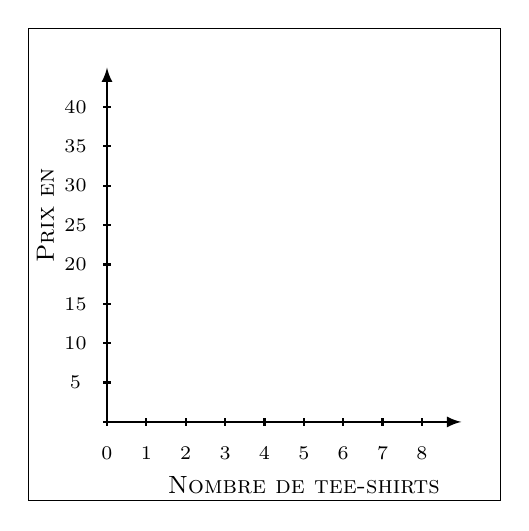
\begin{tikzpicture}[scale=1]
            % Correction
            % Axes
            \draw[thick,>=latex,->](0,0)--+(4.5,0);
            \draw[thick,>=latex,->](0,0)--+(0,4.5);
            \foreach \x in {0,0.5,...,4} \draw[thick] (\x,-.05) -- (\x,0.05);
            \foreach \y in {0,0.5,...,4} \draw[thick] (-.05,\y) -- (0.05,\y);
            \foreach \x / \label in {0/{0} , 0.5/{1}  , 1/{2}  , 1.5/{3} , 2/{4}  , 2.5/{5}  , 3/{6} , 3.5/{7} , 4/{8}} \draw (\x,-0.4) node {\scriptsize\label};
            \foreach \y / \label in { 0.5/5 , 1/10  , 1.5/15  , 2/20 , 2.5/25  , 3/30, 3.5/35, 4/40} \draw (-0.4,\y) node {\scriptsize\label};
            % Label axes
            \node[label={[text depth=-1ex,rotate=90]{\sc\small Prix en \Prix{}}}] at (-0.55,2.5) {};
            \node[label={[text depth=-1ex]below:{\sc\small Nombre de tee-shirts}}] at (2.5,-0.45) {};	
            \tkzSetUpPoint[shape=cross, color=blue];
            \tkzDefPoints{0.5/0.5/A,1/1/B,1.5/1.5/C,2/2/D,2.5/2.5/E,3/3/F,3.5/3.5/G};
            \tkzDrawPoints(A,B,C,D,E,F,G);
            \tkzSetUpPoint[shape=cross, color=DarkGreen];
            \tkzDefPoints{1.5/1.2/H,3/2.4/I};
            \tkzDrawPoints(H,I);        
            % Fond
            \draw (-1,-1) rectangle (5,5);
            \papierMillimetre
        \end{tikzpicture}
        \item Placer, en bleu, les points correspondant à la situation normale et, en vert, les points correspondant à la situation des soldes.
        \item Dans les deux cas, justifier si les prix sont proportionnels au nombre de tee-shirts.
        \item \par\textcolor{red}{Dans les deux cas, les points sont alignés avec l'originie, donc les prix sont proportionnels au nombre de tee-shirts.}
    \end{enumerate}
\end{corrige}

